\documentclass{article}

\usepackage{amsmath,amssymb}
\usepackage{tikz,tkz-tab}
\usetikzlibrary{calc}

\begin{document}
    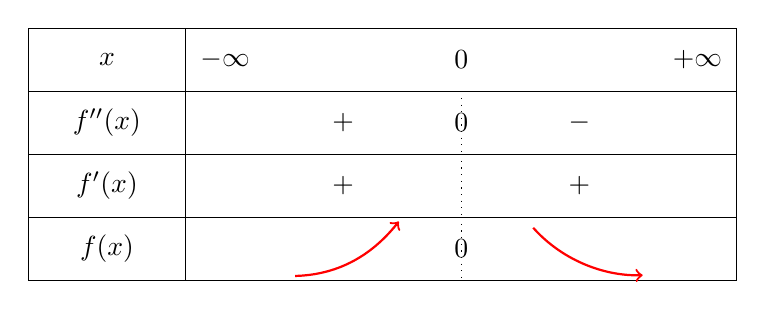
\begin{tikzpicture}
    \tkzTabInit{$x$ /.8 , $f''(x)$ /.8, $f'(x)$/.8 , $f(x)$/.8}{$-\infty$, $0$ , $+\infty$};
    \tkzTabLine{,+,z,-}
    \tkzTabLine{,+,t, +}
    \tkzTabLine{,,z,}
    \draw[red,thick,->,shorten >= 2pt,shorten <= 4pt] ($.5*(N14) + .5*(M14) + (0,.5mm)$) to [bend right=25] ($.5*(N23) + .5*(M13)$);
    \draw[red,thick,->,shorten >= 7pt,shorten <= 7pt] ($.5*(N23) + .5*(M23) + (0,.5mm)$) to [bend right=25] ($.7*(N34) + .3*(M24) + (0,.7mm)$);
\end{tikzpicture}

\end{document}